

\documentclass[twocolumn,10pt]{article}

\usepackage[utf8]{inputenc}

 \usepackage[T1]{fontenc}
\usepackage{xcolor}
\usepackage{float}
\usepackage{graphicx}
\usepackage{siunitx}
\usepackage{geometry}
\usepackage{float}
\usepackage[toc,page]{appendix}
\graphicspath{ {./figuren/} }
\usepackage{fancyvrb}
\usepackage{hyperref}
\hypersetup{
    colorlinks = true,
    linkcolor = blue,
    citecolor=blue,
    linkbordercolor = {white},
}
\usepackage{fullpage}
\usepackage{fancyvrb}
\graphicspath{ {./figuren/} }

\geometry{
    a4paper,
    left=20mm,
    right=20mm,
    top=25mm,
    bottom=25mm,
}

\frenchspacing
\usepackage{booktabs}
\usepackage{microtype}

\usepackage[english,dutch]{babel}

\usepackage{listings}
\lstset{
    belowcaptionskip=1\baselineskip,
    breaklines=true,
    columns=flexible,
    basicstyle=\small\ttfamily,
}
\usepackage{graphicx}
\usepackage{placeins}

\usepackage{xcolor}
\usepackage{titlesec}
\titleformat{\section}[block]{\color{blue}\Large\bfseries\filcenter}{}{1em}{}
\titleformat{\subsection}[hang]{\bfseries\filcenter}{}{1em}{}

\usepackage{mathtools}

\title{Opdracht 1, Algoritmiek}
\author{Jenny Vermeltfoort, s3787494, groep PO1\_20}

\begin{document}

\selectlanguage{dutch}
\def\tablename{Tabel}

\maketitle

\section*{Uitleg}
Cryptarithm is een puzzel waarbij er waardes worden toegekend aan de letters van drie verschillende woorden. Het doel is om een unieke waarde toe te kennen aan elke unieke letter zodat de som van de eerste twee woorden leidt tot de som van het derde woord. Er mogen in deze oplossing geen leading nullen staan. 

Dit document beschrijft de implementatie van een backtracking algoritme om cryptarithmische puzeels op te lossen. De implementatie kan ook bepalen hoeveel unieke puzzels (puzzels met maar 
\'e\'en oplossing) er geconstrueerd kunnen worden met twee woorden.

\section*{Implementatie}

\subsection*{Zoek oplossing}
Om zoek\_oplossing voor te bereiden worden er uit alle worden op de volgorde zoals beschreven in de figuur hieronder uit de woorden gehaald. Voor elke letter wordt bijgehouden in welke kolom de letter voor het eerst voorkomt. 

In de zoek\_oplossing implementatie wordt de p->letters[] lijst op volgorde toegekend. De puzzel wordt per kolom ($K0.. K_n$) geverifieerd. Dit wordt gedaan met een achterlopende kolom index. Wanneer bijvoorbeeld de letter 'O' wordt toegekend uit het voorbeeld hieronder zal kolom K0 worden geverifieerd. Dit wordt gedaan door de waarde van E te berekenen, alle waardes hiervoor zijn bekend ($\text{waarde letter woord0} + \text{waarde letter woord1} + \text{carry}_{K0}$). Deze waarde moet niet al toegekend zijn aan een andere letter, en als de letter E als is toegekend dan moet de toegekende waarde hetzelfde zijn als de waarde die is berekend met de waardes uit de kolom. Is dit niet het geval gaat de implementatie een stapje terug. Bij letter 'B' in het voorbeeld worden de kolommen K1 en K2 geverifieerd op dezelfde manier als hierboven voordat B wordt toegekend.

De linkse letter van het het laatste woord kan al bepaald worden wanneer de lengte van dit woord groter is als beide voorgaande woorden. Deze waarde is namelijk \'e\'en en de carry van deze kolom is ook 1.

Wanneer alle waardes zijn toegekend wordt gecontroleerd of er geen leading nullen zijn en of de carry van de laatste kolom niet 0 of 1 is afhankelijk van het lengte verschil van woord2 en woord0/woord1.

Oorspronkelijk had ik een implementatie gemaakt waarbij alle kolommen waar een letter in zitten bij toekenning werden gecontroleerd. Hiervoor werd per kolom gekeken of er genoeg informatie bekend was om de bepalen of de puzzel nog een oplossing heeft (De carry$_{K(n+1)}$ kon al bepaald zijn bijvoorbeeld, hierdoor moeten de waardes van $K_n$ minimaal samen groter dan het grondgetal zijn. Of heel simpel voor alle toegekende kolommen de som van het derde woord berekenen en kijken of dit nog beschikbaar is.) Hierdoor werd de tijdcomplexiteit minder, echter werdt de logica per iteratie aanzienlijk cpu-cycle zwaar (veel branching en weining ruimtelijke localiteit voor caching, daarbij een hogere cache miss rate) wat leidde tot langere iteratie tijden. Er was hier waarschijnlijk nog wel wat optimalisatie te winnen, echter ben ik persoonlijk tevreden met de huidige implementatie.

\begin{figure}[H]
    \centering
    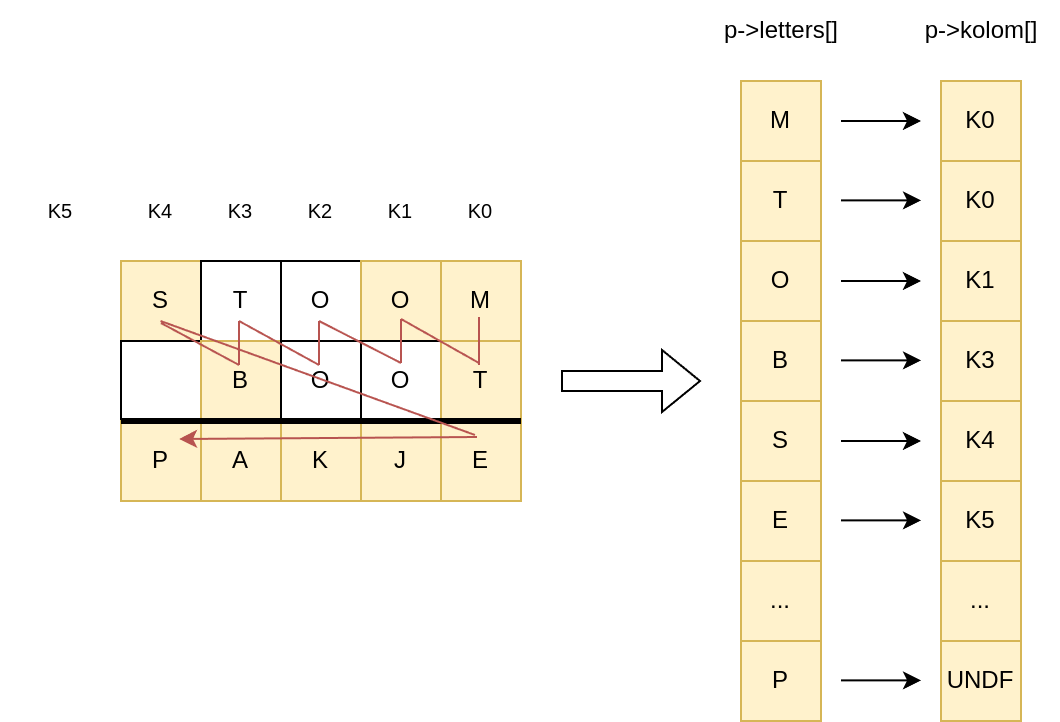
\includegraphics[width=1.0\columnwidth]{letter.png}
        \caption{Sorteer orde.}
    \end{figure}
    \hfill


\subsection*{Construeer puzzel}



\section*{Puzzel oplossingen}

\begin{table}[h]
    \centering
    \caption{Resultaten van verschillende puzzels.}
    \resizebox{\columnwidth}{!}{ % Verklein de tabel naar de kolombreedte
        \begin{tabular}{@{}ccccc@{}}
            \toprule
            Puzzel & Grondgetal & Oplossingen & Bekeken & Tijdsduur \\ 
            \midrule
            STOOM+BOOT=PAKJE & 10 & 5      & 1099 & \SI{29}{\micro\second} \\
            SINT+PIET=RUZIE & 9 & -1       & 229 & \SI{5}{\micro\second} \\
            SINT+PIET=RUZIE & 10 & 16      & 397 & \SI{14}{\micro\second} \\
            SINT+PIET=RUZIE & 11 & 64      & 859 & \SI{21}{\micro\second} \\
            SINT+PIET=RUZIE & 20 & 11068   & 40482 & \SI{883}{\micro\second} \\
            SINT+PIET=RUZIE & 26 & 53590   & 162415 & \SI{3264}{\micro\second} \\
            SINT+PIET=RUZIE, N=3, P=21 & 26 & 213 & 733  & \SI{13}{\micro\second} \\
            \bottomrule
        \end{tabular}
    }
\end{table}
\FloatBarrier

\section*{Puzzel constructies}

\begin{table}[h]
    \centering
    \caption{Resultaten van verschillende constructies.}
    \resizebox{\columnwidth}{!}{ % Verklein de tabel naar de kolombreedte
        \begin{tabular}{@{}cccc@{}}
            \toprule
            Woorden & Grondgetal & Puzzels & Tijdsduur \\ 
            \midrule
            SINT+PIET=... & 10 & 840 & \SI{0.184}{\second} \\
            KLAAS+PAARD=... & 10 & 24864 & \SI{6.074}{\second} \\
            MIJTER+MANTEL=... & 10 & 461320 & \SI{103.948}{\second} \\
            \bottomrule
        \end{tabular}
    }
\end{table}
\FloatBarrier



\begin{appendices}
    \section*{Experimenten Logs}
    \begin{lstlisting}

        De puzzel kent 5 verschillende oplossing(en).
        Het zoeken van de oplossingen kostte 28 clock ticks, ofwel 2.8e-05 seconden.
        We hebben daarbij 1099 deeloplossingen bekeken.
        Een gevonden oplossing is:
        M=2 T=7 O=5 B=8 S=3 E=9 J=0 K=1 A=6 P=4
        Grontgetal: 10 
        Puzzel:
        0: STOOM
        1: BOOT
        2: PAKJE
        Toegekende letters:

        De puzzel kent -1 verschillende oplossing(en).
        Het zoeken van de oplossingen kostte 5 clock ticks, ofwel 5e-06 seconden.
        We hebben daarbij 229 deeloplossingen bekeken.
        Grontgetal: 9 
        Puzzel:
        0: SINT
        1: PIET
        2: RUZIE
        Toegekende letters:
        R=1; 

        De puzzel kent 16 verschillende oplossing(en).
        Het zoeken van de oplossingen kostte 14 clock ticks, ofwel 1.4e-05 seconden.
        We hebben daarbij 397 deeloplossingen bekeken.
        Een gevonden oplossing is:
        T=2 N=5 E=4 I=9 S=6 P=3 Z=8 U=0 R=1
        Grontgetal: 10 
        Puzzel:
        0: SINT
        1: PIET
        2: RUZIE
        Toegekende letters:
        R=1; 

        De puzzel kent 64 verschillende oplossing(en).
        Het zoeken van de oplossingen kostte 21 clock ticks, ofwel 2.1e-05 seconden.
        We hebben daarbij 859 deeloplossingen bekeken.
        Een gevonden oplossing is:
        T=2 N=6 E=4 I=10 S=7 P=8 Z=9 U=5 R=1
        Grontgetal: 11 
        Puzzel:
        0: SINT
        1: PIET
        2: RUZIE
        Toegekende letters:
        R=1; 

        De puzzel kent 11068 verschillende oplossing(en).
        Het zoeken van de oplossingen kostte 883 clock ticks, ofwel 0.000883 seconden.
        We hebben daarbij 40482 deeloplossingen bekeken.
        Een gevonden oplossing is:
        T=2 N=3 E=4 I=7 S=5 P=15 Z=14 U=0 R=1
        Grontgetal: 20 
        Puzzel:
        0: SINT
        1: PIET
        2: RUZIE
        Toegekende letters:
        R=1; 

        De puzzel kent 53590 verschillende oplossing(en).
        Het zoeken van de oplossingen kostte 3264 clock ticks, ofwel 0.003264 seconden.
        We hebben daarbij 162415 deeloplossingen bekeken.
        Een gevonden oplossing is:
        T=2 N=3 E=4 I=7 S=5 P=21 Z=14 U=0 R=1
        Grontgetal: 26 
        Puzzel:
        0: SINT
        1: PIET
        2: RUZIE
        Toegekende letters:
        R=1; 

        De puzzel kent 213 verschillende oplossing(en).
        Het zoeken van de oplossingen kostte 13 clock ticks, ofwel 1.3e-05 seconden.
        We hebben daarbij 733 deeloplossingen bekeken.
        Een gevonden oplossing is:
        T=2 N=3 E=4 I=7 S=5 P=21 Z=14 U=0 R=1
        Grontgetal: 26 
        Puzzel:
        0: SINT
        1: PIET
        2: RUZIE
        Toegekende letters:
        N=3; P=21; R=1; 

        # echo "2 10 SINT PIET 3 4 3" | ./WoordSomPuzzel
        We vonden 840 puzzels met een unieke oplossing.
        Het construeren van de puzzels kostte 184744 clock ticks, ofwel 0.184744 seconden.
        Een mogelijk woord 2 met een unieke oplossing: TTNSN

        # echo "2 10 KLAAS PAARD 3 4 3" | ./WoordSomPuzzel
        We vonden 24864 puzzels met een unieke oplossing.
        Het construeren van de puzzels kostte 6074723 clock ticks, ofwel 6.07472 seconden.
        Een mogelijk woord 2 met een unieke oplossing: SSSDDK

        # echo "2 10 MIJTER MANTEL 3 4 3" | ./WoordSomPuzzel 
        We vonden 461320 puzzels met een unieke oplossing.
        Het construeren van de puzzels kostte 103947895 clock ticks, ofwel 103.948 seconden.
        Een mogelijk woord 2 met een unieke oplossing: RRRREIJ

        
    \end{lstlisting}
 

\end{appendices}

\end{document}